\documentclass[10pt,letterpaper]{article}
\usepackage[margin=1in]{geometry}
\usepackage[T1]{fontenc}
\usepackage{lmodern,microtype,amsmath,amssymb,amsthm,booktabs,array,graphicx,xurl}
\usepackage[hidelinks]{hyperref}
\usepackage{enumitem}
\microtypesetup{protrusion=false}
\setlist{nosep,leftmargin=*}
\setlength{\parskip}{3pt}
\setlength{\parindent}{1em}
\newtheorem{theorem}{Theorem}
\newtheorem{lemma}[theorem]{Lemma}
\newtheorem{proposition}[theorem]{Proposition}
\newtheorem{corollary}[theorem]{Corollary}
\newcommand{\ind}{\mathbf 1}
\newcommand{\R}{\mathbb R}
\newcommand{\dist}{\operatorname{dist}}
\newcommand{\D}{\mathcal D}
\newcommand{\F}{\mathcal F}
\title{Certified Expression Intervals under Shared Segmentation Uncertainty}
\author{Arnav Peram\\[3pt]\normalsize Arizona College Preparatory High School\\\normalsize\texttt{arnavperam1@gmail.com}}
\date{}
\begin{document}
\hypersetup{pdftitle={Certified Expression Intervals under Shared Segmentation Uncertainty},pdfauthor={Arnav Peram},pageanchor=false}
\begin{titlepage}\maketitle\thispagestyle{empty}
\begin{abstract}\normalsize
A shared cell-boundary error can alter several expression counts together in imaging-based spatial transcriptomics. We introduce GeoCert, an exact method for determining which observed cell-by-gene counts remain invariant under a physical boundary-deformation budget and which can change. For ordered boundaries subject to slope, band, thickness and nuclear constraints, one polynomial-size rational cut represents the minimum continuous deformation of every feasible molecular assignment. In the single-interface point-transcript setting, an exact critical-height construction yields a polynomial-time count dynamic program that recovers outcomes missed by every penalty bound. Disjoint boundary ribbons combine into one topology-preserving tissue partition, and min-plus composition allocates a shared area budget across them. A finite union of complete atlases admits alternative ribbon widths while retaining every primary feasible boundary. On Xenium lung crops and a breast format-test dataset, five atlas families per crop yield 496,604 exact interval rows over 17 budgets. At 4 \textmu m\texttwosuperior{}, their union widens 298 lung and 3,595 breast intervals relative to the primary atlas. Across the budget grid, shared geometry tightens independent-molecule outer bounds for 29 of 102 lung and 791 of 2,076 breast questions whose outer width reaches at least two. Under the primary atlas, a separate 600 \textmu m square yields 1,223,400 exact interval rows over eight budgets for 3,171 complete cells. Attaining boundaries certify each interval endpoint and reveal when several molecular transfers share one deformation. GeoCert turns a specified segmentation uncertainty model into exact expression-count intervals and inspectable geometric witnesses.
\end{abstract}
\end{titlepage}
\hypersetup{pageanchor=true}\setcounter{page}{1}

\begin{figure}[t]\centering
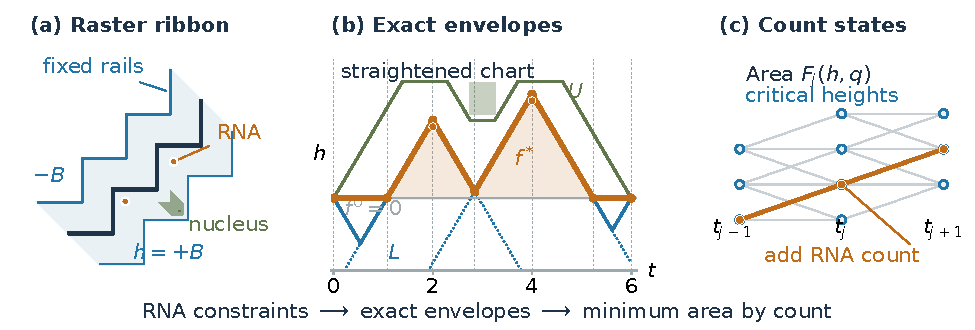
\includegraphics[width=\textwidth]{figures/geometry_pipeline.pdf}
\caption{From a shared boundary to an exact count spectrum (schematic). A shear chart straightens the staircase interface. Molecular requirements generate Lipschitz envelopes; their clamp of the reference minimizes area. Critical heights yield a count-indexed path computation. Theorem~\ref{thm:glue} converts chart displacement to physical area and glues local witnesses.}\label{fig:geometry}
\end{figure}

\section{Introduction}
Imaging-based spatial transcriptomics assigns detected molecules to cells through a segmentation. Which counts can change when a boundary moves? Several molecules may share one deformation or require incompatible boundaries. Independent molecule scores omit these dependencies, and separate local analyses can describe incompatible tissue partitions.

For a reference segmentation and an explicit deformation family, we compute the smallest and largest retained counts attainable within an area budget. Each answer contains a count interval, its geometric assumptions and attaining boundaries. A singleton certifies invariance within that family; a wider interval quantifies count sensitivity.

GeoCert preserves exact joint-assignment area while eliminating continuous boundary coordinates, then composes local changes into one tissue partition under one budget. Theorem~\ref{thm:cost} represents the full assignment-cost function $D^\star(c)$ by a rational cut, supporting general unary objectives and coupled interfaces. For one interface with point transcripts, Theorem~\ref{thm:chain} uses the same canonical minimum-area boundary to compute all attainable counts, including states missed by penalized cuts. Ribbon homeomorphisms make local witnesses globally compatible (Figure~\ref{fig:geometry}). A finite union of complete atlases admits alternative widths while retaining every primary-model deformation.

\paragraph{Relationship to existing methods.}
Baysor, Proseg, BIDCell and Segger estimate segmentation or transcript assignments~\cite{baysor,proseg,bidcell,segger}. ResolVI models downstream misassignment probabilistically~\cite{resolvi}; ovrlpy examines three-dimensional signal overlap~\cite{ovrlpy}. TISSUE constructs uncertainty intervals for predicted, unmeasured expression~\cite{tissue}. Our intervals instead range over geometric alternatives for already observed molecules. They complement these estimators by quantifying sensitivity to a specified family of geometric changes.

Convex segmentation and ordered-label cuts~\cite{hochbaum,ishikawa}, interacting-surface graphs~\cite{li,shah}, higher-order energy constructions~\cite{kz,kohli}, Lipschitz extensions~\cite{petrakis}, and difference-potential lattices~\cite{felsner} provide foundations. Submodularity alone is insufficient for a binary graph representation with auxiliary variables~\cite{zivny}. We prove the particular cost-preserving elimination below. Exact critical heights offer another realization of that reduction; count augmentation uses established resource-state dynamic programming~\cite{hassin}. Our contribution is the continuous assignment-cost identity and its compatible hard-budget realization.



\section{Exact elimination of continuous boundary costs}\label{sec:engine}
We first establish the continuous assignment-cost identity for one moving interface, the building block of the evaluated atlas. Supplement~\S1 extends the construction to multiple ordered interfaces with heterogeneous slopes and minimum/maximum thickness constraints.

\subsection{Requirements and feasible assignments}
Let a boundary $f:I\to\mathbb R$ on a compact rational interval be $s$-Lipschitz, lie in $[\underline b,\overline b]$, and have fixed endpoints. The rational piecewise-affine reference $f^0$ obeys these geometric constraints. A site $i$ is a rectangle $[x_i^-,x_i^+]\times I_i$, including a point as a degenerate case. All sites in group $g(i)$ have one owner $c_g\in\{0,1\}$, with bit $b_g=\ind[c_g=0]$. Clearance $\rho>0$ requires
\begin{equation}
 b_{g(i)}=1\Rightarrow f(t)\ge\ell_i=x_i^++\rho,\qquad
 b_{g(i)}=0\Rightarrow f(t)\le u_i=x_i^--\rho\quad(t\in I_i).\label{eq:owners}
\end{equation}
Nuclear regions are fixed-label groups. They have the same geometric requirements and zero molecular reward. The reference can satisfy the geometry without satisfying every uncertain site's assignment requirement.

\begin{lemma}[Propagation on one interface]\label{lem:kernel}
A lower interval requirement $f\ge\ell_i$ on $I_i$ implies
$f(t)\ge\ell_i-s\dist(t,I_i)$ everywhere. An upper requirement analogously implies $f(t)\le u_i+s\dist(t,I_i)$.
\end{lemma}
\begin{proof}
Apply the Lipschitz inequality between $t$ and the closest point of the closed interval $I_i$. The displayed bounds are attained by the corresponding tent profiles in the absence of other restrictions.
\end{proof}

Forbid a lower activation if $\ell_i>\overline b$ or $\ell_i>f^0(e)+s\dist(e,I_i)$ at either endpoint $e$. Forbid an upper activation if $u_i<\underline b$ or $f^0(e)>u_i+s\dist(e,I_i)$. Add structural pins and
\begin{equation}
 b_{g(i)}\Rightarrow b_{g(j)}\quad\hbox{when}\quad
 \ell_i-s\dist(I_i,I_j)>u_j .\label{eq:imp}
\end{equation}
This implication excludes simultaneous activation of the incompatible lower and upper requirements.

\begin{theorem}[Exact assignment feasibility]\label{thm:feas}
The finite unary restrictions, implications and structural pins characterize the assignments realizable by the continuous family.
\end{theorem}
\begin{proof}
Necessity follows from Lemma~\ref{lem:kernel}. For sufficiency, form the maximum $L$ of the active lower tents, the lower band and both endpoint lower cones. Form the minimum $U$ of the active upper tents, upper band and endpoint upper cones. The pair tests ensure every lower contribution is at most every upper contribution: $\dist(t,I_i)+\dist(t,I_j)\ge\dist(I_i,I_j)$. Unary tests handle bands and endpoints. Thus $L\le U$. Both envelopes are $s$-Lipschitz, satisfy bands and endpoint equality, and realize the selected requirements. They supply continuous feasible boundaries.
\end{proof}

\subsection{Preserving every assignment's minimum area}
For complete owners $c$, write $\mathcal F(c)$ for the realizing boundaries and
\begin{equation}
 D^\star(c)=\min_{f\in\mathcal F(c)}\int_I|f-f^0|\,dt,\qquad \min\varnothing=+\infty.\label{eq:dstar}
\end{equation}
The later chart supplies its physical-area conversion. Shared movement makes this function nonadditive across transcripts.

\begin{theorem}[Assignment-wise cost representation]\label{thm:cost}
For rational input, one polynomial-size rational graph with assignment vertices $b(c)$, auxiliary vertices $y$, logical hard arcs and a known constant $\kappa$ satisfies
\begin{equation}
\min_y\operatorname{Cut}_{G_D}(b(c),y)+\kappa=D^\star(c)\label{eq:identity}
\end{equation}
for every feasible assignment. Hard-feasible cuts exist exactly for realizable assignments. After adding arbitrary rational unary molecular costs and a rational $\lambda\ge0$, a minimum cut detects infeasibility or returns optimal owners and an attaining rational piecewise-affine boundary.
\end{theorem}
\begin{proof}
Scalar minimum and maximum preserve the slope, band and endpoint constraints. Consequently
\begin{equation}
f^*(t)=\min\{U(t),\max\{L(t),f^0(t)\}\}\label{eq:clamp}
\end{equation}
is feasible. Every realization lies between $L$ and $U$, so this clamp is pointwise nearest to $f^0$ and minimizes its integrated displacement.

The positive displacement is the maximum of activated functions $[\ell_i-s\dist(t,I_i)-f^0(t)]_+$. Negative displacement uses upper requirements and complementary bits. Retain fixed requirements and all uncertain-site requirements, including source-inconsistent ones. At feasible owners, positive and negative displacement cannot both occur at the same point. Split at affine-piece endpoints, source knots, zeros and pair crossings. On a slab, sort the positive heights $h_1\ge\cdots\ge h_k>0$, with $h_{k+1}=0$. If $S_j$ contains the activation labels of the first $j$ heights, then
\begin{equation}
\max_{i\ \mathrm{active}}h_i=\sum_{j=1}^k(h_j-h_{j+1})\ind[S_j\hbox{ has an active label}].\label{eq:layers}
\end{equation}
Integrate each nonnegative affine difference exactly. Standard OR helpers encode these weighted activation sets; the complementary polarity reverses the construction~\cite{kz,kohli}. Repeated group labels are a single bit. Mandatory terms become forced helpers or the constant $\kappa$. Minimizing auxiliaries therefore gives the integrated clamp for each fixed $b(c)$, proving~\eqref{eq:identity} before molecular costs are specified. Add unary costs by successive differences, shifting negative terms by a recorded constant. Scale rational capacities to integers. Set each numerical hard capacity above the sum of finite capacities \emph{after} the costs and $\lambda$ are chosen. A hard arc in the optimum certifies infeasibility; otherwise~\eqref{eq:clamp} reconstructs a realizing boundary.
\end{proof}

\paragraph{What elimination contributes.}
For $M$ constant-piece excursion profiles, relative order changes $O(M^2)$ times. Each adjacent swap changes one prefix, giving $O(M^2+M)$ distinct activation helpers after merging. With $G$ groups and $N$ molecular/structural sites, the graph has $O(G+M^2+M)$ vertices and $O(G+N^2+M^2+M)$ arcs. Intersections and integrated weights have polynomial rational encoding. An event sweep~\cite{bentley} accumulates unchanged layer integrals lazily; its construction bound is detailed in Supplement~\S3. The contribution is the exact continuous minimum-area identity represented by these finite gadgets.

The coupled extension propagates constraints through boundary-separation paths before forming its envelopes. Their componentwise min/max closure makes the clamp simultaneously feasible, preserving the same identity for every assignment of $m+1$ labels. Its graph-size and proof details are in Supplement~\S1. The cut representation supports general molecular objectives and coupled boundaries. For the scalar point-transcript atlas, Section~\ref{sec:counts} instead augments the canonical clamp's exact critical mesh with count states, solving hard budgets directly without a Lagrangian gap.

\section{From local interfaces to one compatible tissue model}\label{sec:atlas}
An \emph{atlas} specifies one compatible uncertainty model for the tissue: disjoint two-label ribbons around reference interfaces, with fixed endpoint traces and outer rails. Each RNA belongs to at most one ribbon; the rest of the partition stays fixed. Cell-count outputs for that atlas refer to this single family.

Let $P_i$ be closed ribbons with pairwise disjoint interiors and injective charts $\Psi_i:I_i\times[-B_i,B_i]\to P_i$. The reference boundary is transverse coordinate zero, each half lies wholly in its stated reference label, and each RNA belongs to at most one ribbon. An allowed displacement $h_i$ is continuous, zero at both endpoints, and $|h_i|\le qB_i$ for $q<1$. Fixed regions have additional label constraints.

\begin{samepage}
\begin{theorem}[Compatible gluing and additive physical area]\label{thm:glue}
Every tuple of admissible ribbon boundaries is induced by one global homeomorphism of the reference partition, identity outside the ribbon interiors. For constant chart Jacobians $J_i>0$, the physical area whose label changes is exactly $\sum_i J_i\int|h_i|$.
\end{theorem}
\end{samepage}
\begin{proof}
For fixed $t$, define a map of $[-B_i,B_i]$ by
\begin{equation}
H_i(t,v)=\begin{cases}
-B_i+(v+B_i)(h_i(t)+B_i)/B_i,&v\le0,\\
h_i(t)+v(B_i-h_i(t))/B_i,&v\ge0.
\end{cases}\label{eq:homeo}
\end{equation}
The two positive slopes are bounded away from zero; both branches meet at $h_i(t)$ and have continuous explicit inverses. The map fixes rails and is identity at the interval endpoints. Conjugating $(t,v)\mapsto(t,H_i(t,v))$ by $\Psi_i$ gives a homeomorphism fixing the entire ribbon boundary. Extend by identity outside. Finitely many such maps and inverses agree on intersections, so they glue continuously and bijectively. Cell topology and fixed junction incidences are preserved. The changed-label region in one ribbon lies between zero and $h_i(t)$, with chart area $\int|h_i|$. Change of variables and disjoint interiors give the sum.
\end{proof}

\paragraph{Exact chart for a raster interface.}
For a coordinate-monotone raster-edge path choose $s_x,s_y\in\{-1,1\}$ and let $t=s_xx+s_yy$, $u=s_xx-s_yy$ in pixel coordinates. The exact source arc is $u=r_i(t)$. With pixel size $p$,
\begin{equation}
\Psi_i(t,h)=\frac p2\big(s_x(t+r_i(t)+h),\ s_y(t-r_i(t)-h)\big),\qquad J_i=p^2/2,\label{eq:chart}
\end{equation}
up to the recorded origin. This shear preserves the staircase interface exactly, with constant Jacobian away from measure-zero corners. The optimization variable is displacement $h$, with zero source. Intersecting nuclear pixels impose exact conservative interval constraints that preserve their owners.

This family accommodates arbitrary reference adjacency by fixing junction neighborhoods and uncovered perimeter portions. Its topology and coverage are explicit parts of the uncertainty model.



\section{Hard budgets without assignment enumeration}\label{sec:counts}
For a retained count $N_{kg}(c)$, define the minimum-area spectrum
\begin{equation}
S_{kg}(q)=\min_{c:N_{kg}(c)=q}D^\star(c),\quad
[L_{kg}(\delta),U_{kg}(\delta)]=\left[\min,\max\right]\{q:S_{kg}(q)\le\delta\}.\label{eq:interval}
\end{equation}
The notation means the smallest and largest elements of the displayed feasible-count set. Its interior need not contain every integer. A witness for each endpoint proves attainment; an empty set is reported separately.

\subsection{Exact critical heights and a count chain}
For one boundary, collect all propagated lower/upper requirement pieces, fixed geometric pieces and source pieces before selecting owners. A common mesh contains all piece endpoints and crossings, including source crossings and every point observation. At node $t_j$, retain their candidate values $V_j$ within forced envelopes and discard values violating any point's clearance gap or fixed constraint.

\begin{lemma}[Exact scalar critical mesh]\label{lem:mesh}
Restricting nodal heights to these candidates, enforcing original adjacent slope and ownership constraints, and charging trapezoidal absolute displacement preserves $D^\star(c)$ for every feasible assignment.
\end{lemma}
\begin{proof}
Between consecutive events all candidate pieces are affine and their ordering is fixed. The canonical clamp~\eqref{eq:clamp} selects one such piece and has constant-sign displacement. Its nodal candidates are retained and its trapezoidal area equals its exact integral. Conversely a feasible candidate-height path interpolates to a feasible continuous boundary: every constraint endpoint is in the mesh, and the intervening constraints are linear. The trapezoid upper-bounds that interpolant's absolute-displacement integral, which is at least $D^\star(c)$. The retained canonical minimizer attains equality.
\end{proof}

\begin{samepage}
\begin{theorem}[Polynomial exact spectra for explicit point RNAs]\label{thm:chain}
Assume one boundary, one point per free RNA group, arbitrary fixed structural intervals, and a nonnegative integer per-point count score. Let $W$ be its variable range and $H_j=|V_j|$. Given the critical mesh and its local node scores, the count dynamic program uses $O((W+1)\sum_jH_j)$ arithmetic transition operations and returns every minimum-area count, with backpointers to attaining boundaries. With explicit unit transcripts the complete algorithm is polynomial in the input and rational encoding.
\end{theorem}
\end{samepage}
\begin{proof}
A permitted height at a point's mesh node uniquely determines its owner, since the clearance gap was excluded. Count each observation once at that node. Let $z_j(h)$ be its local score and $a_j(h)=w_j|h-f^0(t_j)|$, where $w_j$ is half the sum of adjacent mesh lengths. Define
\begin{equation}
F_j(h,q)=a_j(h)+\min_{u\in V_{j-1}:|u-h|\le s(t_j-t_{j-1})}
F_{j-1}(u,q-z_j(h)).\label{eq:dp}
\end{equation}
Initialization accounts for fixed groups and the first node. The shortest-path induction gives the exact nodal minimum for every count. Lemma~\ref{lem:mesh} gives continuous equality, including unsupported penalty outcomes. For each predecessor count, allowed sorted predecessors form a sliding interval as $h$ increases. A monotone queue computes its minima in $O(H_{j-1}+H_j)$ operations. Sum over counts and nodes. Backpointers reconstruct candidates and hence attaining boundaries.
If $P$ is the total affine-piece count, a full mesh has $O(P^2+P)$ nodes and $O(P)$ candidates per node; this and rational intersection arithmetic give polynomial preparation and encoding. For unit RNA scores, $W$ is bounded by the explicit molecule count. Binary-compressed multiplicities instead give a pseudo-polynomial count dependence. Free interval-valued RNA groups and arbitrary coupled height vectors require additional state and are outside this scalar result.
\end{proof}

Resource-state shortest paths are standard~\cite{hassin}. Here the critical-mesh proof supplies exact continuous costs for each resource state, rather than treating a user-chosen mesh as exact. Single-copy queries use a cheaper corollary: when the source satisfies every source-owner and structural constraint at zero cost, propagate requested bits, keep unforced source bits, and reconstruct the clamp. Every costly requirement in that completion is forced in all feasible completions, so it is minimum-area. The count-chain theorem does not require this stronger source-assignment premise.

\subsection{One area allowance for the entire atlas}
For a fixed cell and gene, compute each incident patch's spectrum $S_i(d)$ in \emph{count changes} relative to its source. Let $n^0_{kg}$ include all retained RNA in that reference cell, including outside the ribbons. Then
\begin{equation}
S_{kg}(q)=\min_{d_1+\cdots+d_r=q-n^0_{kg}}\sum_{i=1}^r S_i(d_i).\label{eq:convolution}
\end{equation}
This is min-plus convolution. An attaining trace selects one witness per patch, and Theorem~\ref{thm:glue} gives a valid global partition. Conversely every allowed partition decomposes into patch states costing at least their local minima. These two directions prove~\eqref{eq:convolution}. Patches with no relevant gene can stay at their zero-cost source. A simple convolution takes $O(rW^2)$ operations. Thus scalar point-RNA patch atlases give polynomial exact single-cell/gene spectra despite arbitrary fixed reference adjacency.

No molecule or exterior count is duplicated, and $\delta$ is spent once. Every allowed full count matrix lies componentwise inside the table, but different rows' endpoints need not coexist. Joint marker questions require vector spectra or a joint predicate query, rather than multiplying marginal endpoint sets.

\subsection{Alternative complete atlases}
Width-specific atlases can offer different feasible deformations. Their union preserves these alternatives without requiring their supports to be nested.

\begin{proposition}[Exact finite-family certificates]\label{thm:union}
Let $\mathcal F_1,\ldots,\mathcal F_A$ be complete atlas families with the same reference partition, counted observations and physical-area cost. If $S_a(q)$ is the exact count spectrum of member $a$, then the family $\mathcal F_\cup=\bigcup_{a=1}^A\mathcal F_a$ has spectrum
\begin{equation}
 S_\cup(q)=\min_a S_a(q).\label{eq:union}
\end{equation}
Every finite minimum inherits an attaining boundary and its member identity. At budget $\delta$, $L_\cup=\min_a L_a$ and $U_\cup=\max_a U_a$, omitting members with empty feasible-count sets; the union is empty exactly when all members are empty.
\end{proposition}
\begin{proof}
Each partition in the union belongs to a member and costs at least that member's minimum for its count. Conversely, a member attaining the least finite minimum supplies a partition in the union at that cost. Taking the extreme budget-feasible counts proves the endpoint identities.
\end{proof}
Merging costs $O(\sum_a|\operatorname{dom}S_a|)$ comparisons after member spectra are computed. Each witness selects one complete atlas, with its own compatible ribbons. Including the primary family preserves its feasible states and fixed-key reference-count reach. Joint predicates use the same member selection; mixing patches across members would define a different model.

\subsection{Why a penalty path alone is insufficient}
An exact cut yielding $m(\mu)=\min_c\{\mu D^\star(c)-N(c)\}$ gives
\begin{equation}
U(\delta)\le\left\lfloor\mu\delta-m(\mu)\right\rfloor,\qquad\mu\ge0.\label{eq:dual}
\end{equation}
This is weak duality. Feasible witnesses give the opposite bound; a gap is retained unless exact refinement closes it. Applying the same argument to $-N$ bounds the lower endpoint.

A gap occurs even with eight \emph{distinct, explicit unit} transcripts. Take source zero on $[0,30]$, slope one, band $[-4,4]$, and clearance $1/10$. At longitudinal centers $5,15,25$, place clusters of $2,3,3$ RNAs. In a cluster of height $a=2,3,3$, respectively, point $j$ is $(t,x)=(\mathrm{center}+j/100,a-j/100-1/10)$. Clearance forces common ownership within each cluster; its first cone dominates, and cluster supports are disjoint. The exact count/area states are $(0,0),(2,4),(3,9),(5,13),(6,18),(8,22)$. At budget ten the maximum is three, whereas the best penalty upper bound is four: for $\mu\le1/3$, the count-eight state gives $B(\mu)\ge8-12\mu\ge4$; for $\mu\ge1/3$, the count-two state gives $B(\mu)\ge2+6\mu\ge4$. Equality holds at $1/3$. The count chain recovers the unsupported count-three state. The example uses no binary-encoded multiplicity.

\section{Evaluation: count effects and geometric reach}\label{sec:eval}
\subsection{Observed inputs and fixed extraction rules}
Two lung crops contain 7,370 retained Q20 measured-gene records from one public Xenium specimen~\cite{data,xenium}. Eligible cells are connected and avoid crop borders. Interfaces between eligible cells or an eligible cell and background are traced into monotone arcs of four to 128 edges, with one frozen edge at each end. The primary atlas processes longer arcs first and tries chart support halfwidths $B=4,2,1,1/2$, accepting the first feasible width. Exact intersection tests certify side labels and disjoint interiors. The displacement band is $|h|\le3B/4$, slope limit one, and clearance $10^{-6}/p$. Nuclear fragments retain fixed owners; Supplement~\S2 specifies the extraction rules.

The same rule is applied to two Xenium breast crops containing 81,182 retained RNAs, from the vendor's trimmed two-FOV format-test dataset~\cite{breasttest}. This second input tests transfer of the geometric construction and exact computation. Table~\ref{tab:scope} summarizes both atlases.

\begin{table}[ht]\centering
\begin{tabular}{lrr}\toprule
Quantity&Lung crops&Breast crops (Xenium)\\\midrule
Retained RNA&7,370&81,182\\
Crop-contained connected cells&153&467\\
Disjoint ribbons&544&1,708\\
RNA inside ribbons&745&8,262\\
Editable incident-edge coverage&68.3\%&65.8\%\\
Cell--gene spectra&3,304&22,976\\
Original eight-budget interval rows&26,432&183,808\\\bottomrule
\end{tabular}
\caption{Primary-atlas size and coverage. All eligible reference cells contribute to coverage, including cells with no editable arc. Count spectra include positive or editable cell--gene pairs; RNA outside the ribbons contributes its fixed reference count.}\label{tab:scope}
\end{table}

\subsection{Certified invariance and shared-boundary count changes}
The exact spectra yield 210,240 interval rows on budgets $0,0.05,0.1,0.25,0.5,1,2,4\,\mu\mathrm m^2$. At budget $4$, 2,780/3,304 lung counts (84.1\%) and 17,717/22,976 breast counts (77.1\%) are certified invariant within the primary atlas. At budget $0.05$, these fractions are 88.9\% and 84.0\%. The remaining intervals quantify count variation and provide attaining boundaries. These totals include fixed counts outside editable ribbons.

A marginal outer bound allows every individually affordable transfer simultaneously. A feasibility-matched additive inner approximation instead charges the sum of singleton transfer areas. The first can overspend the common budget or combine incompatible choices; the second can omit affordable shared movement.

A joint-count difference requires a question with at least two individually movable transcripts. We therefore also report question-level denominators: across the original budget grid, marginal width is at least two in 46 lung and 1,026 breast cell--gene questions. Exact geometry tightens 4/46 (8.7\%) and 203/1,026 (19.8\%), respectively, affecting 4/153 and 139/467 eligible cells. Across all questions, these fractions are 4/3,304 (0.12\%) and 203/22,976 (0.88\%). The corresponding tightened \emph{row} counts remain four and 228; additive-inner missed endpoints remain two and 68. On the finer 17-budget grid, the same spectra tighten 12/46 lung questions (26.1\%) and 361/1,026 breast questions (35.2\%), capturing differences that occur between the original budget samples (Supplement~\S7).

In breast cell 81, LDHB has retained source count 22. At area $0.25\,\mu\mathrm m^2$, the exact interval is $[19,23]$ versus marginal $[17,23]$. At area $0.5$, it is $[17,23]$ versus additive-inner $[18,23]$. An attaining boundary transfers three LDHB molecules through one ribbon and two through another, plus one collateral KRT8 molecule. The physical areas are approximately $0.342327$ and $0.141713\,\mu\mathrm m^2$, totaling $0.484040$. This witness demonstrates both approximation failures within the same geometry (Figure~\ref{fig:witness}).

\begin{figure}[t]\centering
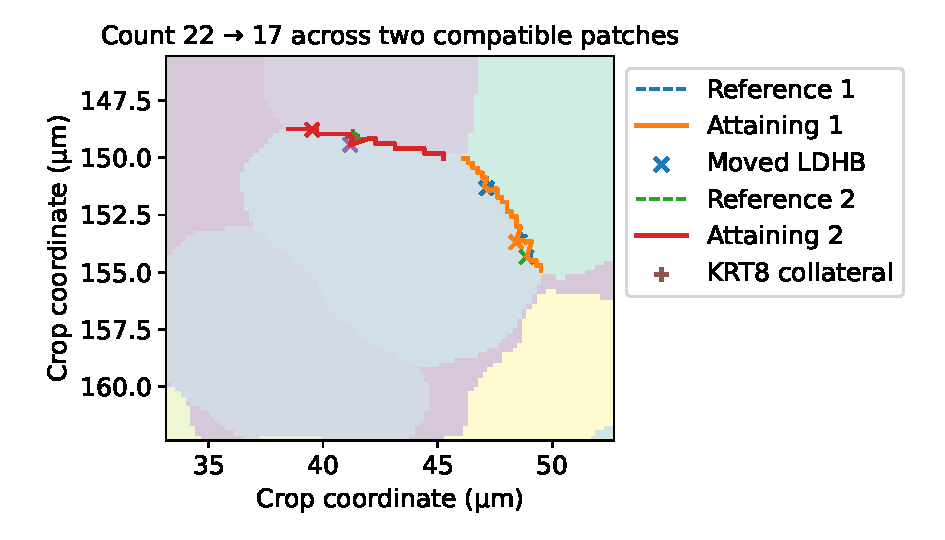
\includegraphics[width=.93\textwidth]{figures/cell_witness.pdf}
\caption{Original reference mask and a count-17 LDHB witness across two compatible patches. Crosses mark five transferred LDHB molecules; the plus marks collateral KRT8. Both changes spend one physical-area budget and coexist in the same partition.}\label{fig:witness}
\end{figure}

\paragraph{Joint marker co-detection.}
A joint predicate can ask whether both EPCAM and PTPRC remain detected in one cell under the same deformation. At budget $0.25\,\mu\mathrm m^2$, five of seven initially co-detected lung cells and 46 of 48 breast cells retain co-detection throughout the primary atlas family; the remaining two in each dataset admit a witness that removes it. These primary-atlas joint certificates persist through budget $4$ (Supplement~\S8.4), illustrating how the same geometry answers a multi-gene question.

\subsection{Budget-dependent variation and saturation}
The primary support cap $B\le4$ and pixel pitch $p\simeq0.2125\,\mu\mathrm m$ imply a maximum paired-coordinate displacement of
\begin{equation}
 \|\Psi(t,h)-\Psi(t,0)\|_2\le\frac{3pB}{4\sqrt2}\le0.4508\,\mu\mathrm m.\label{eq:cap}
\end{equation}
Nuclear and endpoint constraints can further restrict this submicrometre allowance.

From area $0.25$ onward, non-singleton totals remain 524 in lung and 5,259 in breast, although 61 breast intervals widen by $0.5$ and three more by $1$. The last endpoint thresholds are approximately 0.240525 and 0.573939, respectively. Area therefore controls attainable counts even after interval occupancy stabilizes; Supplement~\S6 gives the full budget tables.

\subsection{Wider ribbons: reach versus coverage}\label{sec:reach}
Before computing width-study outcomes, we fixed support halfwidths $r=0.5,1,2,3\,\mu\mathrm m$ and 17 area budgets from 0 to 16. Each run keeps the original paths, ordering, nuclei, seams and slope. Its required chart halfwidth is $B=\lfloor4\sqrt2r/p\rfloor/4$, with no narrower fallback. These separately extracted atlases obey the same chart and gluing proof and isolate the effect of wider supports.

At support 3, the displacement cap reaches $2.226\,\mu\mathrm m$, while coverage falls to 16.9\% in lung and 17.8\% in breast (Table~\ref{tab:reach}). Local gene multiplicity reaches 17 and last endpoint thresholds reach 4.878 and 13.783$\,\mu\mathrm m^2$. Third-cell interfaces and ribbon conflicts reject more wide supports. The adaptive extractor retains narrow ribbons where needed; fixed-width extraction disables this fallback.

\begin{table}[ht]\centering
\begin{tabular}{lrrrrr}\toprule
Support&Displacement&\multicolumn{2}{c}{Edge coverage (\%)}&Lung Proseg&Breast nuclear\\
halfwidth&cap ($\mu$m)&Lung&Breast&reach (\%)&reach (\%)\\\midrule
Adaptive&0.451&68.3&65.8&6.6&16.2\\
0.5&0.366&45.1&44.6&4.3&11.2\\
1&0.733&33.8&34.6&5.5&14.8\\
2&1.493&23.5&24.7&4.5&14.6\\
3&2.226&16.9&17.8&3.8&12.2\\
\bottomrule\end{tabular}
\caption{Required physical support halfwidths are rounded down to quarter chart units. The cap is $3pB/(4\sqrt2)$; actual feasibility also depends on other constraints. Reach is the fraction of changed reference counts attainable at any budget, with fixed denominators across families.}\label{tab:reach}
\end{table}


All five families are evaluated on the same 17-budget grid. The supplement reports each family's interval occupancy, endpoint changes and joint-geometry effects at every budget.

\subsection{Reach of independent reference assignments}
An image-only reference assigns each RNA to the nearest labelled nuclear pixel within $5\,\mu\mathrm m$, or to background. A five-micrometre crop-edge guard avoids relying on unseen nuclei. We also analyze Proseg 3.2.0 executions~\cite{proseg} on both lung crops. The default factorization failed on the small first crop; one completed stochastic run per crop used factorization disabled, otherwise retaining upstream sampler settings. Proseg assigned 43.0\% and 90.1\% of returned molecules to background in the two crops. The comparison tests a broader reassignment regime than local boundary motion. Transcript joins and original-cell mapping were checked against both saved count matrices.

All widths use the same eligible cell--gene comparison keys, excluding keys affected by reference-missing RNA in any member. This gives 2,798 changed Proseg entries, and 1,114 lung and 10,965 breast nuclear-reference changes. The primary and widest families attain the fractions in Table~\ref{tab:reach}; replacing the adaptive atlas with wider uniform supports reduces aggregate reach (Figure~\ref{fig:reach}).

\begin{figure}[t]\centering
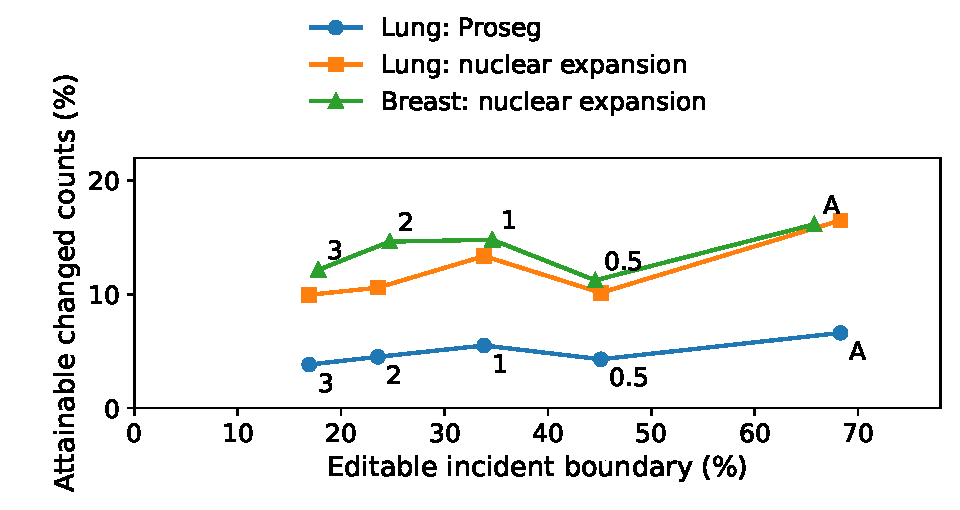
\includegraphics[width=.90\textwidth]{figures/reach_coverage.pdf}
\caption{Unbounded-budget count reach versus editable incident-edge coverage on fixed comparison keys. Labels give required support halfwidth in micrometres; A denotes the original adaptive-width atlas. Lines connect separately extracted families, rather than a nested sequence. Proseg is one adapted execution per clipped lung crop. }\label{fig:reach}
\end{figure}

\subsection{Combining width alternatives}
Within each crop, we apply Proposition~\ref{thm:union} to the primary atlas and the four fixed-width families, using the same observations, reference cells and area units. Each endpoint selects one complete member atlas. Table~\ref{tab:union-reach} shows the resulting increase in countwise reach: 130 additional Proseg changes in lung, 115 additional lung nuclear-reference changes and 1,169 additional breast nuclear-reference changes become attainable. These alternatives retain the primary atlas's narrow-ribbon deformations while admitting motions up to the widest member's $2.226\,\mu\mathrm m$ cap where its supports permit them.

\begin{table}[ht]\centering
\begin{tabular}{lrrr}\toprule
Reference&Changed keys&Primary attainable&Union attainable\\\midrule
Lung: Proseg&2,798&185 (6.6\%)&315 (11.3\%)\\
Lung: nuclear&1,114&184 (16.5\%)&299 (26.8\%)\\
Breast: nuclear&10,965&1,773 (16.2\%)&2,942 (26.8\%)\\\bottomrule
\end{tabular}
\caption{Countwise attainability without an area cap, on identical comparison keys. The union chooses among five complete atlases and contains every primary-atlas state.}\label{tab:union-reach}
\end{table}

On the same 3,304 lung and 22,976 breast questions used for the primary atlas, the union certifies 2,524 (76.4\%) and 15,143 (65.9\%) counts as invariant at area $4$, compared with the primary 84.1\% and 77.1\%. At this budget, 298 lung and 3,595 breast intervals widen. The full union census contains 29,212 questions and 496,604 rows across 17 budgets (Supplement~\S5). Across this grid, shared geometry tightens the envelope of member-wise independent-molecule bounds for 29/102 lung (28.4\%) and 791/2,076 breast (38.1\%) questions whose outer interval reaches width at least two.

The union's intervals answer a broader sensitivity question than any one width setting. Gains reflect alternative patch selection as well as displacement range. Coverage remains member-specific: its largest local displacement and largest covered boundary fraction need not occur in the same atlas. Each complete reference assignment remains outside the union because every member excludes it. Attainable count entries can require different witnessing partitions.

\subsection{Correctness and operating range}
An independent scalar/Cartesian implementation reproduces all 210,240 primary interval rows. Width-study witnesses pass continuous checks, all compositions and interval rows are rechecked, and 246 hash-selected multicopy questions agree with independent scalar enumeration. These checks share prepared geometry; Proseg execution records are checked separately. A separate implementation reconstructs all 29,212 union spectra and 496,604 interval rows and checks their selected witnesses. The supplement gives the complete verification scope.

Three fresh processes per size solve an analytical equal-tent family, computing every count and checking its boundary. Median complete times for 16, 32, 64 and 128 explicit RNAs are 0.465, 1.574, 7.138 and 42.206 seconds. At 128, the method visits 605,632 height/count states and recovers all 129 levels of the closed-form spectrum without enumerating $2^{128}$ assignments (Supplement~\S9).

The primary adaptive atlas also completes on prespecified $400$ and $600\,\mu\mathrm m$ breast squares with 1,363 and 3,171 complete cells, producing 554,224 and 1,223,400 exact interval rows. The $400\,\mu\mathrm m$ run uses the count chain and takes 22.55 minutes for extraction, geometry validation and count/witness computation. The $600\,\mu\mathrm m$ run uses exact enumeration; measured attempt time is 36.89 minutes, including an initial deadline interruption and count-only retry. Independent output audits confirm all rows and witness counts and areas (Supplement~\S9).

\section{Discussion and availability}
The reduction separates a molecular count question from the least continuous geometry realizing it. Critical heights retain exact minima under count constraints, while compatible ribbons make local witnesses jointly interpretable within a single reference partition. The LDHB example shows why independent transfer permissions and additive transfer costs can err in opposite directions. The width study separates local displacement from covered boundary length. A finite union retains the deformations of all five models and increases reference-count reach with inherited exact witnesses. Reporting the selected atlas alongside each endpoint makes that broader family explicit.

\paragraph{Limits.}
The certificates are exact for the specified family. Each atlas member fixes seams and uncovered boundaries while preserving topology and nuclear ownership. Anatomical calibration of slopes, widths and budgets is a separate empirical task. The evaluation uses two lung crops from one donor, a breast format-test input intended for computational testing, and one adapted Proseg execution per clipped lung crop; these assess computation and sensitivity rather than assignment accuracy or downstream biological validity. Generalization across donors and whole-slide scaling remain open. Different interval endpoints may require different partitions, so multi-gene conclusions use joint queries. Extending hard-budget count computation to moving junctions and coupled interfaces is a natural next step.

\paragraph{Software and disclosure.}
The MIT-licensed companion contains the atlas implementation, exact spectra, source crops, Proseg records and reproducible analyses. The source, inputs and results are at \url{https://github.com/arnavperam/geocert/tree/f1e5dbb29c96d6b014508ce7f1eb1abcfb490190/recomb2027-atlas}. The release record identifies the separately rebuilt manuscript and supplement. Source data retain 10x CC BY 4.0 attribution. Generative AI assisted mathematical development, algorithm design, implementation, experiments, verification and writing. The author is responsible for the claims and submission.

\clearpage
\begin{thebibliography}{99}
\bibitem{baysor} V. Petukhov et al. Cell segmentation in imaging-based spatial transcriptomics. \emph{Nature Biotechnology} 40:345--354, 2022. doi:10.1038/s41587-021-01044-w.
\bibitem{proseg} D. C. Jones, A. E. Elz, A. Hadadianpour, H. Ryu, D. R. Glass, and E. W. Newell. Cell simulation as cell segmentation. \emph{Nature Methods} 22:1331--1342, 2025. doi:10.1038/s41592-025-02697-0.
\bibitem{li} K. Li, X. Wu, D. Z. Chen and M. Sonka. Optimal surface segmentation in volumetric images---a graph-theoretic approach. \emph{IEEE TPAMI} 28(1):119--134, 2006. doi:10.1109/TPAMI.2006.19.
\bibitem{shah} A. Shah, M. D. Abr\`amoff and X. Wu. Optimal surface segmentation with convex priors in irregularly sampled space. \emph{Medical Image Analysis} 54:63--75, 2019. doi:10.1016/j.media.2019.02.004.
\bibitem{mcshane} E. J. McShane. Extension of range of functions. \emph{Bulletin of the American Mathematical Society} 40(12):837--842, 1934. doi:10.1090/S0002-9904-1934-05978-0.
\bibitem{whitney} H. Whitney. Analytic extensions of differentiable functions defined in closed sets. \emph{Transactions of the American Mathematical Society} 36(1):63--89, 1934. doi:10.2307/1989708.
\bibitem{kz} V. Kolmogorov and R. Zabih. What energy functions can be minimized via graph cuts? \emph{IEEE TPAMI} 26(2):147--159, 2004. doi:10.1109/TPAMI.2004.1262177.
\bibitem{data} 10x Genomics. Preview Data: FFPE Human Lung Cancer with Xenium Multimodal Cell Segmentation. Xenium Onboard Analysis 2.0.0 (preview), 5 February 2024. CC BY 4.0. \url{https://www.10xgenomics.com/datasets/preview-data-ffpe-human-lung-cancer-with-xenium-multimodal-cell-segmentation-1-standard}.
\bibitem{xenium} 10x Genomics. Understanding Xenium Outputs. Xenium Onboard Analysis 2.0 documentation. \url{https://www.10xgenomics.com/support/software/xenium-onboard-analysis/2.0/analysis/xoa-output-understanding-outputs}. Accessed 31 October 2026.
\bibitem{felsner} S. Felsner and K. Knauer. Distributive lattices, polyhedra, and generalized flows. \emph{European Journal of Combinatorics} 32(1):45--59, 2011. doi:10.1016/j.ejc.2010.07.011.
\bibitem{resolvi} C. Ergen and N. Yosef. ResolVI: addressing noise and bias in spatial transcriptomics. \emph{Nature Methods} 23:2003--2014, 2026. doi:10.1038/s41592-026-03212-9.

\bibitem{hochbaum} D. S. Hochbaum. An efficient algorithm for image segmentation, Markov random fields and related problems. \emph{Journal of the ACM} 48(4):686--701, 2001. doi:10.1145/502090.502093.
\bibitem{ishikawa} H. Ishikawa. Exact optimization for Markov random fields with convex priors. \emph{IEEE TPAMI} 25(10):1333--1336, 2003. doi:10.1109/TPAMI.2003.1233908.
\bibitem{kohli} P. Kohli, L. Ladick\'y and P. H. S. Torr. Robust higher order potentials for enforcing label consistency. \emph{International Journal of Computer Vision} 82:302--324, 2009. doi:10.1007/s11263-008-0202-0.
\bibitem{zivny} S. \v{Z}ivn\'y, D. A. Cohen and P. G. Jeavons. The expressive power of binary submodular functions. \emph{Discrete Applied Mathematics} 157(15):3347--3358, 2009. doi:10.1016/j.dam.2009.07.001.
\bibitem{bidcell} X. Fu et al. BIDCell: Biologically-informed self-supervised learning for segmentation of subcellular spatial transcriptomics data. \emph{Nature Communications} 15:509, 2024. doi:10.1038/s41467-023-44560-w.
\bibitem{segger} E. Heidari, A. Moorman et al. Segger: Fast and accurate cell segmentation of imaging-based spatial transcriptomics data. \emph{bioRxiv}, 2025. doi:10.1101/2025.03.14.643160.
\bibitem{ovrlpy} S. Tiesmeyer et al. Identifying 3D signal overlaps in spatial transcriptomics data with ovrlpy. \emph{Nature Biotechnology}, published online 10 February 2026. doi:10.1038/s41587-026-03004-8.

\bibitem{bentley} J. L. Bentley and T. A. Ottmann. Algorithms for reporting and counting geometric intersections. \emph{IEEE Transactions on Computers} C-28(9):643--647, 1979. doi:10.1109/TC.1979.1675432.

\bibitem{tissue} E. D. Sun, R. Ma, P. Navarro Negredo, A. Brunet and J. Zou. TISSUE: uncertainty-calibrated prediction of single-cell spatial transcriptomics improves downstream analyses. \emph{Nature Methods} 21:444--454, 2024. doi:10.1038/s41592-024-02184-y.
\bibitem{joksch} H. C. Joksch. The shortest route problem with constraints. \emph{Journal of Mathematical Analysis and Applications} 14(2):191--197, 1966. doi:10.1016/0022-247X(66)90020-5.
\bibitem{breasttest} 10x Genomics. Example Xenium Datasets: Xenium Human Breast Gene Expression (Multimodal), two-FOV test dataset (\nolinkurl{Xenium_V1_human_Breast_2fov}). Xenium Onboard Analysis 2.0. CC BY 4.0. \url{https://www.10xgenomics.com/support/software/xenium-onboard-analysis/2.0/resources/xenium-example-data}. Accessed 31 October 2026.
\bibitem{biologicalbreast} 10x Genomics. FFPE Human Breast with Pre-designed Panel. Xenium Onboard Analysis 1.0.2; ductal and lobular carcinoma donors. CC BY 4.0. \url{https://www.10xgenomics.com/datasets/ffpe-human-breast-with-pre-designed-panel-1-standard}. Accessed 31 October 2026.
\end{thebibliography}

\end{document}
